\documentclass[preprint,11pt]{elsarticle}
\usepackage{graphicx}
\usepackage{booktabs}
\usepackage{amsmath,amssymb}
\usepackage{enumitem}
\usepackage[hidelinks]{hyperref}
\graphicspath{{figs/}}
\journal{Engineering Applications of Artificial Intelligence}

\begin{document}

\begin{frontmatter}
\title{Learning When to Inspect at High Resolution:\\
Visibility-Aware Triage for Fabric Defect Detection}
\author[a]{Kehan Yao\corref{cor1}}
\ead{yaokh1996@hotmail.com}
\author[b]{Haonan Feng}
\cortext[cor1]{Corresponding author}
\address[a]{China Telecom Group Hangzhou Branch, Hangzhou, China}
\address[b]{The Third Research Institute of the Ministry of Public Security, Shanghai, China}
\begin{abstract}
Industrial fabric inspection requires detecting tiny and weakly visible defects
under constrained computation. Low-resolution detectors are efficient but miss
defects whose visual evidence is insufficient, whereas full high-resolution
inference is expensive and may even degrade easy cases due to scale-distribution
shift. This paper proposes a visibility-boundary-aware detection framework for
industrial fabric defect inspection. Through a cross-resolution failure
diagnosis we show that a range of cheap interventions---threshold calibration,
loss reweighting, knowledge distillation, and sparse patch reinspection---fail
to recover visibility-limited misses, because the missing evidence is not
present in the low-resolution input. Guided by this diagnosis, the proposed
framework uses cross-resolution failure supervision to learn which images are
visibility-limited and selectively triggers full-image high-resolution
reinspection only on those, while explicitly separating ambiguous defects that
remain unrecoverable even at high resolution. On a public fabric defect
detection dataset from Science Data Bank, the method recovers about $69\%$ of
the high-resolution recall gain at roughly $63\%$ of its computational cost, and
an oracle triage even exceeds uniform high-resolution inference by retaining
low-resolution inference on easy images. The analysis further reveals that a
large fraction of missed defects are inherently ambiguous or
annotation-sensitive, highlighting practical reliability boundaries for
AI-based fabric inspection.
\end{abstract}

\begin{keyword}
fabric defect detection \sep industrial visual inspection \sep
adaptive-resolution inference \sep cross-resolution failure analysis \sep
reliability-aware detection
\end{keyword}

\end{frontmatter}

\section{Introduction}
\label{sec:intro}

Fabric defect detection is a representative industrial visual inspection task
that demands high recall, low latency, and low computational cost
simultaneously. In production settings, missing a defect is costly, yet
inspection must keep pace with high-throughput manufacturing on commodity
hardware. A central difficulty is that many fabric defects---nep, broken or
hanging warp, weft shrinkage, and weak-texture anomalies---are extremely small
or visually faint, and are easily missed when detectors operate at the low
input resolutions favored for efficiency.

Most prior work treats such misses as a model-capacity problem, addressing them
through network architecture, loss design, knowledge distillation, multi-scale
training, or sliding-window inference. These approaches implicitly assume that a
missed defect could have been detected with a better low-resolution model. They
do not distinguish between a \emph{recoverable} miss---where the evidence is
present but the model is insufficiently sensitive---and a miss caused by
\emph{insufficient input information}, where the defect occupies too few pixels
for any low-resolution model to recover.

We make this distinction concrete through a cross-resolution diagnosis. Running
the same detector at low ($640$) and high ($1280$) resolution partitions missed
defects into three regimes: threshold-suppressed misses recoverable by
calibration; visibility-limited misses recoverable only by genuine high
resolution; and ambiguous misses that persist even at high resolution. We then
show empirically that a range of cheap interventions---per-class threshold
calibration, miss-rate loss reweighting~\cite{focalloss,eql}, a small-object detection head, feature
distillation, and sparse patch reinspection---fail to recover the
visibility-limited misses. Only full-image high-resolution inference recovers
them, but it quadruples cost and, on easy data, can even reduce accuracy.

This motivates treating the problem not as one of improving low-resolution
representation, but as one of \emph{deciding when to pay the high-resolution
cost}. We propose Visibility-Boundary-Aware Detection (VBAD). VBAD constructs a
visibility label automatically from cross-resolution failure agreement
(low-resolution miss followed by high-resolution recovery), trains a lightweight
visibility head on a frozen detector to predict it, and selectively triggers
full-image high-resolution reinspection only on images judged
visibility-limited. It additionally surfaces the ambiguous, unrecoverable
fraction as a reliability boundary for human review.

Our contributions are:
\begin{enumerate}[leftmargin=1.5em]
\item A cross-resolution failure diagnosis for industrial fabric defect
detection, showing that missed defects arise from threshold suppression,
visibility limitation, and ambiguous low-reliability cases, and that cheap
low-resolution interventions empirically fail to recover the visibility-limited
ones.
\item A visibility-boundary-aware detection framework that learns from
cross-resolution failure supervision to selectively trigger full-image
high-resolution reinspection, improving the recall--cost trade-off over both
uniform low- and high-resolution inference.
\item Validation on a public Science Data Bank fabric defect dataset, including
an ambiguity boundary analysis that quantifies how many missed defects are
inherently unrecoverable and should be escalated for manual review.
\end{enumerate}

\section{Related Work}
\label{sec:related}

\paragraph{Fabric and surface defect detection.}
Automated fabric inspection has moved from hand-crafted texture analysis to deep
detectors~\cite{fabricsurvey}. Recent fabric-specific models improve sensitivity
to small and subtle defects through fine-grained convolutions, attention
modules~\cite{cbam}, small-object detection layers, and tiny-object loss
functions~\cite{fabricyolo,liang2025denim}; recent surveys review this rapidly
growing literature~\cite{eaaisurvey}. These methods frame the residual
difficulty as a model-capacity problem and seek a stronger low-resolution
detector; they do not separate misses that are recoverable in principle from
 misses caused by insufficient input resolution.

\paragraph{Small-object and industrial defect detection.}
Small-object detection is a long-standing challenge, addressed through
higher-resolution features, scale-aware training, context, and
augmentation~\cite{sodsurvey,focalloss}. In industrial inspection, benchmarks
span metallic surface defects~\cite{neudet} and unsupervised anomaly
detection~\cite{mvtecad}, and class-imbalance-aware detectors have been
proposed for defects with rare categories~\cite{eaaiimbalance}. Our work is complementary: rather than proposing a
stronger detector or anomaly model, we analyze when input resolution is the
binding constraint and act on that diagnosis.

\paragraph{Object detectors.}
Modern object detection spans two-stage detectors built on region
proposals~\cite{fasterrcnn} and single-stage detectors that regress boxes
directly~\cite{yolov1,ssd}, typically over deep residual
backbones~\cite{resnet} with multi-scale feature
pyramids~\cite{fpn}. We build on standard real-time detectors spanning the
anchor-free YOLO line~\cite{yolov1,yolov8,yolo11} and the
detection-transformer line (DETR~\cite{detr}, Deformable DETR~\cite{deformabledetr}, RT-DETR~\cite{rtdetr}); our
diagnosis and framework treat the detector as a frozen black box and are not
specific to either family.

\paragraph{Resolution, tiling, and adaptive inference.}
High input resolution is a well-known lever for small-object detection, and
sliding-window or tiling schemes such as SAHI~\cite{sahi} process an image at high
resolution in pieces. These apply high resolution \emph{uniformly} (to the whole
image or to a regular grid), incurring large cost. Adaptive-resolution and
coarse-to-fine methods~\cite{ranet,drnet,dynamiczoom} reduce this cost by
selecting where to look or at what resolution to process, typically driven by
objectness, confidence, or a learned resolution predictor. VBAD differs in its supervision:
the trigger is learned from \emph{cross-resolution failure modes}---images where
low resolution demonstrably fails and high resolution demonstrably recovers---
rather than from generic saliency or confidence heuristics, tying the decision
directly to when high resolution is actually worthwhile.

\paragraph{Class imbalance and long-tailed recognition.}
Fabric defect categories are heavily imbalanced. Long-tailed recognition has
been tackled by loss reweighting~\cite{eql,focalloss}, decoupling
representation from classifier learning~\cite{decoupling}, bilateral-branch
architectures~\cite{bbn}, and minority-class augmentation such as
copy-paste~\cite{copypaste}. Our diagnosis shows, however, that on this fabric
benchmark per-class difficulty is governed by visibility rather than frequency,
so frequency-indexed remedies are not the binding lever; we therefore focus on
the resolution dimension.

\paragraph{Detector error analysis.}
Diagnostic toolkits such as TIDE~\cite{errortaxonomy} decompose detector errors
into interpretable types. We instantiate a resolution-centric analysis for
industrial inspection and, unlike purely diagnostic work, turn the analysis into
an operational triage policy and a reliability boundary.

\section{Method}
\label{sec:method}

We first formalize a cross-resolution failure taxonomy derived from the
diagnosis (Section~\ref{sec:taxonomy}), then describe the Visibility-Boundary-Aware
Detection (VBAD) framework (3.2), its visibility head (3.3), and an ambiguity
boundary analysis (3.4).

\subsection{Cross-resolution failure taxonomy}
\label{sec:taxonomy}
Let a detector at input resolution $r$ produce a set of detections $D_r$ for an
image. A ground-truth defect $g$ is \emph{matched} by $D_r$ when some
detection $d \in D_r$ satisfies
\begin{equation}
\mathrm{match}(d, g) \;=\; \big[\,\mathrm{IoU}(d, g) \ge 0.5\,\big] \wedge
\big[\,\mathrm{cls}(d) = \mathrm{cls}(g)\,\big].
\end{equation}
Write $m_r(g) = 1$ if any detection in $D_r$ matches $g$, else $0$. Using a
low-resolution detector ($r{=}640$) and a high-resolution detector
($r{=}1280$), we partition every ground-truth defect into three types:
\begin{align}
\text{Type-N (normal)}:&\quad m_{640}(g) = 1,\\
\text{Type-V (visibility-limited)}:&\quad m_{640}(g) = 0 \;\wedge\; m_{1280}(g) = 1,\\
\text{Type-A (ambiguous)}:&\quad m_{640}(g) = 0 \;\wedge\; m_{1280}(g) = 0.
\end{align}
Type-N defects are already recovered cheaply. Type-V defects are the actionable
set: their visual evidence is insufficient at $640$ but sufficient at $1280$,
so they can be recovered by paying a higher resolution cost. Type-A defects
remain missed even at high resolution; as the per-class analysis in
Section~\ref{sec:exp} shows, these concentrate in extremely small
($<0.05\%$ image area) and weak-texture categories whose annotations are
themselves scale-sensitive, so we treat them as a reliability boundary rather
than an optimization target. Crucially, the Type-V label is obtained
automatically from cross-resolution failure agreement, not from manual
heuristics.

\subsection{VBAD framework}
\label{sec:vbad}
The key engineering question is \emph{when} to pay the high-resolution cost.
Running $1280$ on every image is expensive and, as we show in
Section~\ref{sec:exp}, can even degrade easy images due to scale-distribution
shift. VBAD therefore performs a per-image triage (Fig.~
\ref{fig:framework}):
\begin{enumerate}[leftmargin=1.4em]
\item Run the low-resolution detector to obtain detections $D_{640}$ and a
backbone feature descriptor $\phi$.
\item A lightweight \emph{visibility head} maps $\phi$ to a score
$s_{\mathrm{vis}} \in [0, 1]$ estimating whether the image contains Type-V
defects.
\item If $s_{\mathrm{vis}} \ge \tau$, run the high-resolution detector on the
\emph{full image} and use $D_{1280}$; otherwise keep $D_{640}$.
\end{enumerate}
We deliberately use full-image high-resolution reinspection rather than cropped
patches. A patch-based variant (Section~\ref{sec:exp}) recovers far fewer
defects because cropping discards the global context and scale distribution the
high-resolution detector relies on. Because Type-N and Type-A defects do not
benefit from the switch, and the two classes the framework routes between
(640 vs 1280 outputs) are taken as-is, the merge step is a simple selection and
needs no cross-resolution box fusion.

\subsection{Visibility head}
\label{sec:vishead}
The visibility head is trained as an image-level binary classifier. Its target
is
\begin{equation}
y_{\mathrm{vis}} = \mathbb{1}\big[\,\exists\, g : \text{Type-V}(g) = 1\,\big],
\end{equation}
i.e.\ the image contains at least one Type-V defect. The descriptor $\phi$
concatenates the globally pooled backbone feature of the $640$ detector with
four cheap scalar cues available from the same forward pass: the number of
low-confidence detections (score in $[0.05, 0.25)$, exposing
threshold-suppressed boxes), the number of confident detections, the smallest
predicted box area, and the mean detection confidence. A two-layer perceptron
maps $\phi$ to $s_{\mathrm{vis}}$, optimized with a class-balanced binary
cross-entropy loss
\begin{equation}
\mathcal{L} = \mathrm{BCE}\big(s_{\mathrm{vis}}, y_{\mathrm{vis}}; w_{+}\big),
\end{equation}
where $w_{+}$ reweights the positive class by its inverse frequency. The
detector is \emph{frozen} while the visibility head is trained, isolating the
triage-learning problem from detector optimization and keeping the added cost
of the head negligible relative to a detector forward pass.

\subsection{Ambiguity boundary analysis}
\label{sec:ambiguity}
Beyond triage, VBAD exposes a reliability boundary. The Type-A set---defects
missed even at high resolution---quantifies how many misses are
\emph{inherently unrecoverable} by resolution alone. We report the Type-A
fraction overall and per class, together with object-size and annotation
statistics, as a diagnostic rather than a trained component. In an industrial
inspection setting this boundary is directly actionable: images or classes with
high Type-A rates are precisely those an automated system should escalate to
manual review instead of optimizing against.

\section{Experiments}
\label{sec:exp}

\subsection{Dataset and protocol}
We evaluate on a public fabric defect detection dataset from Science Data
Bank~\cite{scidb_fabric}
(Table~\ref{tab:data}). It contains 21 defect categories over ${\sim}4{,}800$
images with a strongly long-tailed distribution. We freeze the original
validation split as a held-out test set and carve a class-stratified $15\%$ of
the training split for model selection, yielding $3{,}257$ training / $563$
validation / $954$ test images; all reported numbers are on the held-out test
set. Detectors are trained under an identical equal-budget protocol
(200 epochs, batch size 16) at the stated input resolution. We report
COCO-style~\cite{coco} mAP@0.5 and per-group recall (head/medium/tail by training-instance
count), and---for the visibility analysis---per-ground-truth recall at
IoU${=}0.5$. The split and the Type-V/Type-A construction scripts are released
for reproducibility.

\begin{table}[t]
\centering
\caption{Dataset statistics (held-out test set).}
\label{tab:data}
\begin{tabular}{lc}
\toprule
Property & Value \\
\midrule
Defect categories & 21 \\
Train / val / test images & 3{,}257 / 563 / 954 \\
Test ground-truth defects & 1{,}625 \\
Imbalance ratio (head:tail instances) & $1531\times$ \\
Tiny defects ($<0.05\%$ image area) & cls7 66\%, cls17 69\% \\
\bottomrule
\end{tabular}
\end{table}

\subsection{Resolution is effective but not free}
Table~\ref{tab:resolution} reports the effect of input resolution. Raising
resolution from $640$ to $960$--$1280$ lifts mAP from $0.397$ to ${\sim}0.50$
($+10$ points, $0.501{\pm}0.014$ over three seeds at $1280$), and the gain is
consistent across detector families (YOLOv11m@1280${=}0.515$). However, the
benefit saturates: $1536$ does not improve over $1280$. More importantly, on a
near-balanced 4-class control dataset (also from Science Data Bank) the same high-resolution setting
\emph{reduces} mAP from $0.906$ to $0.862$. High resolution is thus effective
for hard, visibility-limited data but wasteful or harmful otherwise---motivating
selective use.

\begin{table}[t]
\centering
\caption{Effect of input resolution (fabric test set). $^\dagger$mean$\pm$std
over three seeds.}
\label{tab:resolution}
\begin{tabular}{lcccc}
\toprule
Resolution & mAP$_{50}$ & $R_\text{head}$ & $R_\text{med}$ & $R_\text{tail}$ \\
\midrule
640 (baseline)     & 0.397 & 0.554 & 0.367 & 0.475 \\
960                & 0.496 & 0.615 & 0.442 & 0.527 \\
1280$^\dagger$     & $0.501{\pm}.014$ & 0.611 & 0.482 & 0.538 \\
1536               & 0.499 & 0.608 & 0.498 & 0.441 \\
\bottomrule
\end{tabular}
\end{table}

\subsection{Cheap interventions fail to recover visibility-limited misses}
Before triage, we ask whether a cheaper alternative to high resolution exists.
Table~\ref{tab:methods} summarizes six low-resolution interventions (with the baseline) trained at $640$. Per-class
threshold calibration trades precision for recall along the existing curve;
miss-rate loss reweighting only redistributes recall (mAP $0.397{\to}0.398$); a
smaller backbone and a P2 small-object head both reduce mAP; feature
distillation from a $1280$ teacher recovers only $+2.4$ points and leaves the
tiny-defect classes unchanged; and a sparse patch-reinspection variant has an
oracle recall of $0.463$, below full $1280$, because cropping discards global
context. None recovers the tiny-defect classes, which require genuine
high-resolution pixels rather than improved low-resolution representation.

\begin{table}[t]
\centering
\caption{Low-resolution interventions on fabric test set. None recovers the
visibility-limited misses; only full high resolution does.}
\label{tab:methods}
\begin{tabular}{lc}
\toprule
Method (input $640$ unless noted) & mAP$_{50}$ \\
\midrule
Baseline                              & 0.397 \\
Per-class threshold calibration       & R$+0.09$ / P$-0.10$ \\
Miss-rate loss reweighting            & 0.398 \\
Smaller backbone (anti-overfit)       & 0.365 \\
P2 small-object head                  & 0.365 \\
Feature distillation ($1280{\to}640$) & 0.421 \\
Sparse patch reinspection (oracle)    & 0.463 \\
\midrule
Full high resolution ($1280$)         & 0.482 \\
\bottomrule
\end{tabular}
\end{table}

\subsection{VBAD triage}
Table~\ref{tab:vbad} and Fig.~\ref{fig:recallcost} report the triage results
at the ground-truth recall level. Full $1280$ raises recall from $0.410$ to $0.572$ but quadruples cost.
An oracle that triggers high resolution exactly on images containing Type-V
defects reaches $0.615$---\emph{above} full $1280$---at only $29\%$ trigger
rate, because retaining $640$ on easy images avoids the high-resolution
degradation. The learned visibility head attains recall $0.52$ at $40\%$
trigger rate (relative cost $2.6\times$ vs.\ $4.0\times$ for full $1280$),
recovering about $69\%$ of the $640{\to}1280$ recall gain at roughly $63\%$ of
the high-resolution cost. The head predicts Type-V images with
AUC${=}0.66$ (Fig.~\ref{fig:roc}); the gap to the oracle reflects that Type-V evidence is only
weakly observable at $640$ (by definition the $640$ detector missed it).

\begin{table}[t]
\centering
\caption{VBAD triage on fabric test set (per-GT recall). Relative cost
counts the $640$ pass on all images plus the $1280$ pass on triggered images
($1280 {\approx} 4{\times}$ the FLOPs of $640$).}
\label{tab:vbad}
\begin{tabular}{lccc}
\toprule
Method & Recall & Trigger & Rel.\ cost \\
\midrule
Low-res $640$            & 0.410 & 0\%    & $1.0\times$ \\
Full high-res $1280$     & 0.572 & 100\%  & $4.0\times$ \\
Simple trigger (min-box) & 0.471 & 30\%   & $2.2\times$ \\
\textbf{VBAD (learned head)} & \textbf{0.521} & 40\% & $2.6\times$ \\
VBAD (oracle)            & 0.615 & 29\%   & $2.2\times$ \\
\bottomrule
\end{tabular}
\end{table}

\subsection{Tiny-defect classes and the ambiguity boundary}
Table~\ref{tab:ambiguity} and Fig.~\ref{fig:taxonomy} examine where recall is lost. For the tiny-defect
classes, high resolution helps substantially (e.g.\ spandex-break
$0.32{\to}0.66$, hanging-warp $0.16{\to}0.56$), confirming the
visibility-limited diagnosis. Yet a large Type-A fraction remains: overall
$42.8\%$ of test defects are missed even at $1280$, rising to $73\%$ (nep) and
$74\%$ (weft-shrink) for the hardest tiny classes. These are dominated by
sub-$0.05\%$-area instances whose annotations are themselves uncertain. Figure~
\ref{fig:examples} shows representative cases. VBAD
surfaces this fraction explicitly, marking it as a reliability boundary for
human review rather than a target for further optimization.

\begin{table}[t]
\centering
\caption{Tiny-defect classes and Type-A (unrecoverable) rate on the fabric dataset test
set. $R_{640}/R_{1280}$ are per-GT recall.}
\label{tab:ambiguity}
\begin{tabular}{lcccc}
\toprule
Class & $n$ & $R_{640}$ & $R_{1280}$ & Type-A \\
\midrule
nep (cls7)            & 33  & 0.18 & 0.27 & 73\% \\
broken-warp (cls10)   & 48  & 0.19 & 0.35 & 65\% \\
hanging-warp (cls11)  & 32  & 0.16 & 0.56 & 44\% \\
weft-shrink (cls13)   & 53  & 0.09 & 0.26 & 74\% \\
spandex-break (cls17) & 149 & 0.32 & 0.66 & 34\% \\
\midrule
All classes           & 1625 & 0.410 & 0.572 & 42.8\% \\
\bottomrule
\end{tabular}
\end{table}


\begin{figure}[t]
\centering
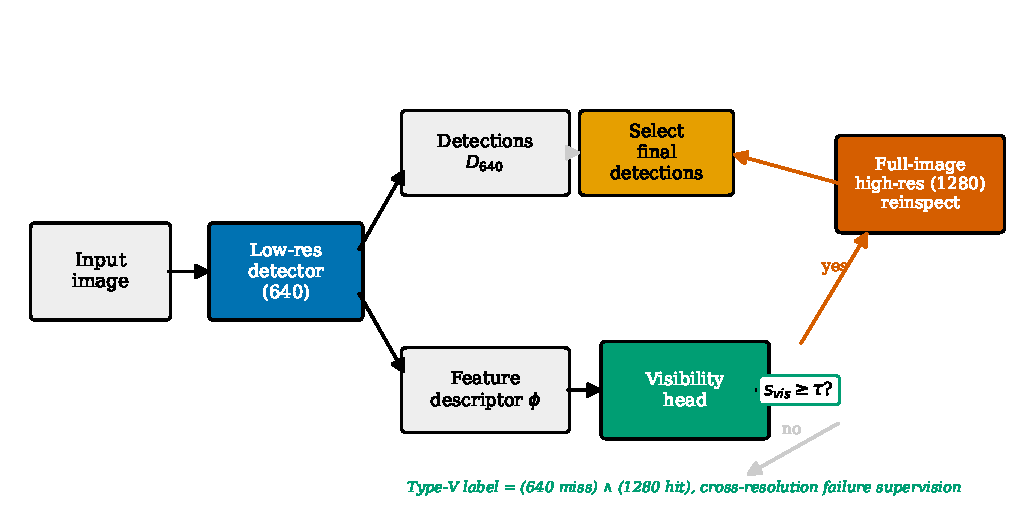
\includegraphics[width=0.95\linewidth]{fig1_framework.pdf}
\caption{The VBAD framework. A frozen low-resolution detector produces
detections and a feature descriptor; a lightweight visibility head, supervised
by cross-resolution failure (Type-V), decides whether to trigger full-image
high-resolution reinspection. Easy images keep the low-resolution result.}
\label{fig:framework}
\end{figure}

\begin{figure}[t]
\centering
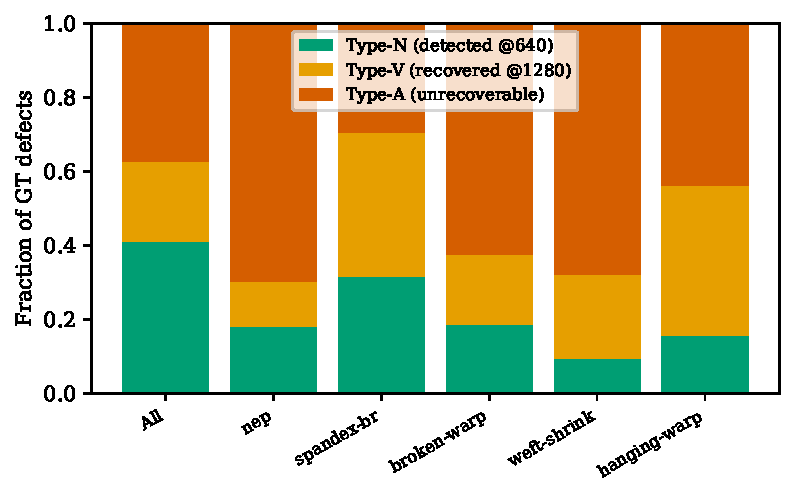
\includegraphics[width=0.7\linewidth]{fig2_taxonomy.pdf}
\caption{Cross-resolution failure taxonomy (test set). For each group, the
fraction of ground-truth defects that are Type-N (detected at $640$), Type-V
(recovered at $1280$), and Type-A (unrecoverable even at $1280$). Tiny-defect
classes are dominated by Type-A.}
\label{fig:taxonomy}
\end{figure}

\begin{figure}[t]
\centering
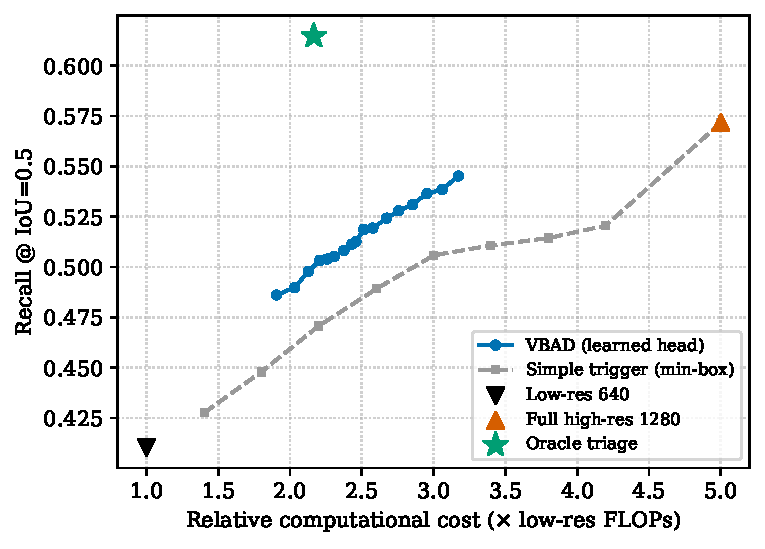
\includegraphics[width=0.72\linewidth]{fig3_recall_cost.pdf}
\caption{Recall--cost trade-off (test set). VBAD dominates the simple min-box
trigger and approaches full high-resolution recall at far lower cost; the oracle
triage exceeds uniform high resolution by retaining low resolution on easy
images.}
\label{fig:recallcost}
\end{figure}

\begin{figure}[t]
\centering
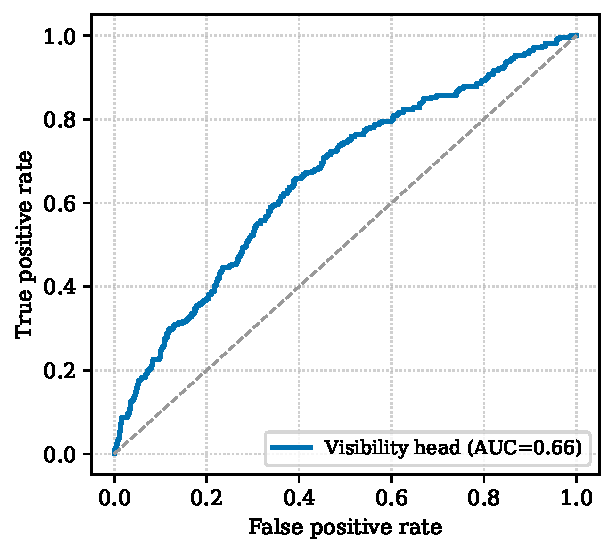
\includegraphics[width=0.55\linewidth]{fig5_roc.pdf}
\caption{Visibility head ROC for predicting Type-V images. The moderate AUC
reflects that Type-V evidence is only weakly observable at $640$.}
\label{fig:roc}
\end{figure}

\begin{figure}[t]
\centering
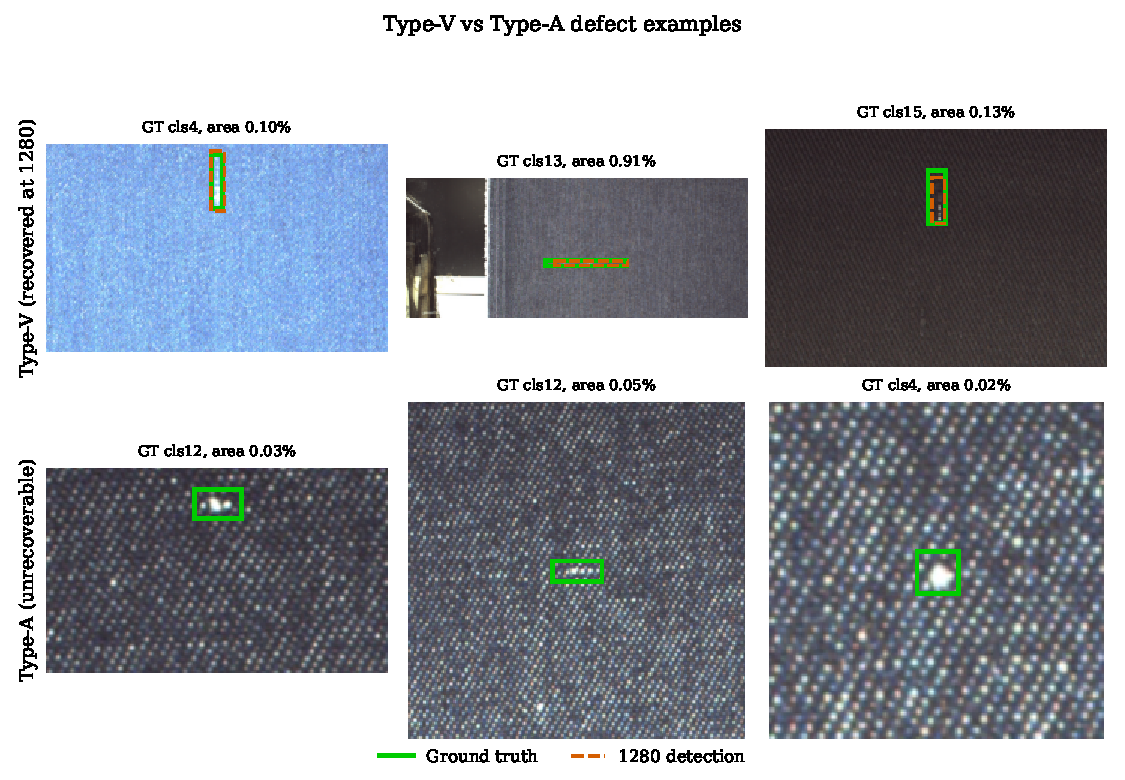
\includegraphics[width=0.92\linewidth]{fig4_examples.pdf}
\caption{Representative Type-V and Type-A defects (test set). Top: Type-V
defects missed at 640 but recovered at 1280 (dashed). Bottom: Type-A defects
missed even at 1280. The latter are faint, sub-pixel-scale anomalies whose
ground-truth annotations are themselves scale-sensitive.}
\label{fig:examples}
\end{figure}

\section{Discussion}
\label{sec:discussion}

\paragraph{Why cheap interventions fail.}
The interventions in Table~\ref{tab:methods} share an implicit assumption: that
a low-resolution model can be made sensitive enough to recover the misses.
Distillation~\cite{kd} aligns a $640$ student to a $1280$ teacher, yet leaves the
tiny-defect classes unchanged---feature alignment cannot reconstruct pixel
evidence that the $640$ input never contained. Patch reinspection does access
more pixels, but cropping removes the global context and scale distribution the
high-resolution detector was trained on, so isolated patches recover few
defects. Both observations point to the same conclusion: for visibility-limited
defects the bottleneck is the input information itself, and only genuine
full-image high resolution supplies it.

\paragraph{Why selective triage helps.}
VBAD does not attempt to circumvent this bottleneck; it decides when to pay for
it. The oracle triage exceeds uniform high resolution because $640$ and $1280$
are complementary: high resolution recovers visibility-limited defects but
slightly harms easy images through scale-distribution shift, so retaining $640$
where it suffices is beneficial. The learned head captures a usable part of this
signal at a fraction of the cost, though a gap to the oracle remains. That gap
is expected: a Type-V defect is by construction one the $640$ detector missed,
so its evidence at $640$ is weak, bounding how well any head conditioned on
$640$ features can anticipate it.

\paragraph{The reliability boundary.}
Perhaps the most consequential finding for deployment is that $42.8\%$ of missed
defects are unrecoverable even at high resolution, concentrated in sub-pixel
classes with scale-sensitive annotations. No resolution policy addresses these;
they define a ceiling on automated recall. An inspection system that reports not
only detections but also \emph{which images lie near this boundary} lets
operators route uncertain cases to manual review---a more honest and practical
behavior than silently optimizing a metric these instances cannot move.

\paragraph{When does VBAD help? A contrasting dataset.}
VBAD is only beneficial when a dataset actually contains visibility-limited
defects. To probe this boundary we apply the same analysis to GC10-DET~\cite{gc10det}, a public
metallic-surface defect benchmark of a different domain (10 classes, 2{,}292
images). Table~\ref{tab:gc10} contrasts the two datasets. On GC10-DET the
low-resolution detector already reaches a high recall ($0.673$), high resolution
yields \emph{no} gain---in fact a slight drop in mAP ($0.657 \to 0.631$)---and
only $8.1\%$ of defects are Type-V, versus $21.5\%$ on the fabric dataset. In
other words, GC10-DET defects are largely visible at low resolution, so there is
little for high-resolution reinspection to recover. The practical consequence is
desirable: a visibility-aware policy triggers high resolution on only a small
fraction of GC10-DET images and therefore neither wastes computation nor incurs
the mild high-resolution degradation. VBAD thus adapts to the dataset---it
contributes where visibility is the bottleneck and stays close to the
low-resolution detector where it is not---rather than applying high resolution
indiscriminately.

\begin{table}[t]
\centering
\caption{When high resolution helps: the fabric dataset is visibility-limited,
the metallic-surface dataset GC10-DET is not. mAP and recall on each test set.}
\label{tab:gc10}
\begin{tabular}{lcc}
\toprule
& Fabric (this work) & GC10-DET \\
\midrule
mAP$_{50}$ @640        & 0.397 & 0.657 \\
mAP$_{50}$ @1280       & 0.482 & 0.631 \\
High-res gain          & $+0.085$ & $-0.026$ \\
Recall @640            & 0.410 & 0.673 \\
Recall @1280           & 0.572 & 0.665 \\
Type-V fraction        & 21.5\% & 8.1\% \\
\bottomrule
\end{tabular}
\end{table}

\paragraph{Limitations.}
Our study uses a single public fabric dataset and two fixed resolutions; the
triage policy is binary rather than a continuous resolution selector, and the
visibility head conditions on global features only. Extending the framework to
multiple resolution tiers, to other surface-inspection domains, and to a
spatially localized visibility map are natural next steps.

\section{Conclusion}
\label{sec:conclusion}

We presented a visibility-boundary-aware approach to fabric defect detection
that reframes resolution as an engineering decision rather than a fixed setting.
A cross-resolution diagnosis separates missed defects into threshold-suppressed,
visibility-limited, and ambiguous types, and shows that cheap low-resolution
interventions empirically fail to recover the visibility-limited ones---only
full-image high resolution does, at a cost that is wasteful or harmful on easy
data. The proposed framework learns from cross-resolution failure supervision
when to trigger full-image high-resolution reinspection, recovering most of the
high-resolution recall gain at a fraction of its cost, and explicitly exposes
the fraction of defects that remain unrecoverable as a reliability boundary for
human review. Rather than claiming to solve tiny-defect detection, the framework
improves the recall--cost trade-off and makes the practical reliability limits
of resolution-limited inspection explicit. Future work includes multi-tier
resolution policies, spatially localized visibility estimation, and validation
across additional surface-inspection domains.


\section*{Data availability}
The fabric defect dataset is publicly available from Science Data Bank~\cite{scidb_fabric}
(DOI: 10.57760/sciencedb.17138). The data split and the
Type-V/Type-A construction scripts are released to support reproduction.

\bibliographystyle{elsarticle-num}
\bibliography{references}

\end{document}
